\section{Method}

\subsection{Creation of RBN-Reservoirs, the perturbing thereof}

RBNs are initialized randomly, and connected to a Ridge regression readout layer \cite{WhatIsRidgeRegression?}.
They are then trained on the tasks from the next subsection.

In literature, one frequently 'perturbs' or 'annoys' RBNs to see how change spreads through the network. \cite{CitationMissing}
RBNs usually don't take input, but we can extend this Perturbation model to make the RBN handle input as follows:

\begin{itemize}
  \item Initialize RBN, set state to all 0's
  \item LoopStart: Set input-connected nodes to input value
  \item Run RBN as CRBN for 1 time-step, logging the RBN state
  \item If input left, goto loopstart, else give all RBN states to next node in flow
\end{itemize}

The Ridge-Regression layer then receives all the intermediate states, as well as what each of the states should be classified as, and attempts to do regression on this dataset.

If the RBN-Reservoir has 'good' dynamics,
the readout layer will be able to correctly classify the input stream.
Such reservoir / readout layers are then stored, or 'pickled' to disk for later analysis and re-use.

\subsection{Tasks}

To measure RBN reservoir performance, a classification task is required.
To simplify IO transformations from and to the reservoir system,
a binary classification task, consisting of binary input data,
where the reservoir consumes one bit at a time, is chosen.

Two such tasks were introduced in \cite{rbn-reservoir}: Temporal Density and Temporal Parity.
Both require the reservoir to be able to retain information for a sliding window of size $ n $,
offset by some value $ t $, back through the input stream.
The temporal Parity task requires us to determine if there were an odd number of ones in the sliding window,
the temporal density task to determine whether there were a majority of ones.
The former is visualized in figure \ref{figure:temporal-parity}.

\begin{figure}
  \subfloat[Input]{
    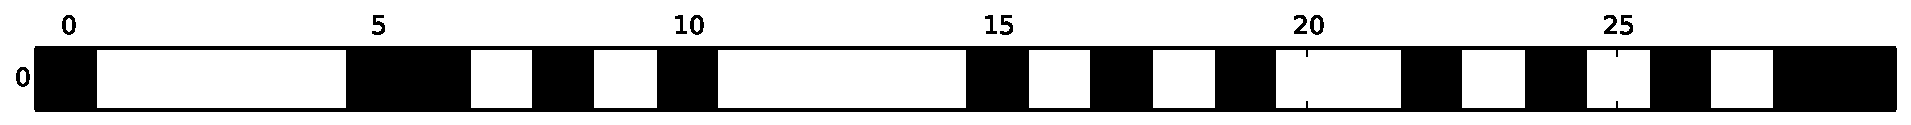
\includegraphics[width=\columnwidth]{method/temporal_parity-10-200-3-input.pdf}
  }

  \subfloat[Correct output]{
    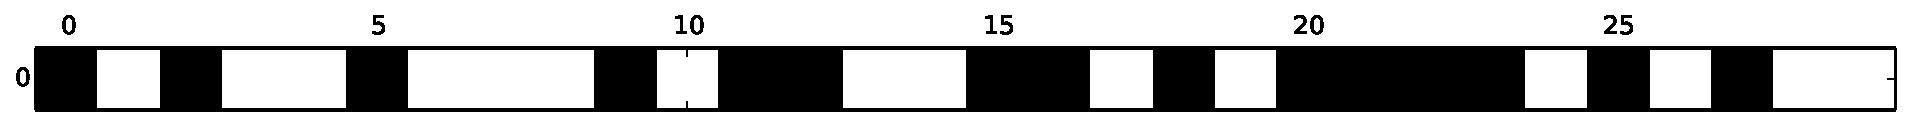
\includegraphics[width=\columnwidth]{method/temporal_parity-10-200-3-output.pdf}
  }

  \caption{
    The first 30 elements of a Temporal Parity task with $[n=3, t=0]$.
    A one is visualized as white, while a zero is black.
    We see that correct output at time $i$ is equal to there being an odd number of $1$s in inputs $[i, i-1, i-2]$
  }
  \label{figure:temporal-parity}
\end{figure}

\subsection{Find some other place for this?}

It seems that for a random sample of reservoirs of a given size and connetivity,
the temporal density task is solveable for a larger $ n $ than the temporal parity one.
The parity task might therefore requires a more specialized network topology to function well.
Due to the seemingly increased complexity of separating the temporal parity task at low $ n $,
it was chosen as the main task in this paper.

%\todo{Talk a bit about required reservoir complexity, as measured in that previous papaer here?}

\subsection{Evolving RBN-Reservoirs}

\begin{itemize}
  \item Here we present how a Genetic Algorithm works
  \item Here we present the Genome used in the task
  \item Here we present the fitness function used
\end{itemize}

Note that we allow variable-input connections, even though the readout-layer was trained on a RBN with fixed number of input-connections.

\subsection{Measuring dynamics}

\begin{itemize}
  \item
    How do i estimate computational power?
    Use the complexity measure from \cite{rbn-reservoir} of course!
  \item
    How do i estimate transient times and attractor lengths?
    Random samling! Link to some algorithm i use here
  \item
    Fun Anecdote: Link to that paper measuring power usage in RBN-Reservoirs:
    \cite{rbn-reservoir-energy-efficiency}
\end{itemize}

\subsection{Weaknesses}

\begin{itemize}
  \item Extremely large state-space
  \item Can be difficult to generalize results
  \item
    Genome representation, inefficient, better with binary string?
    Luckily dominated by RBN-Reservoir simulation time
\end{itemize}


\subsection{Experimental setup}

To verify that RBN simulation is working as expected,
a RBN is created randomly, initial state set to all zeros, and ran.
The results are visualized in figure \ref{figure:rbn-noperturb}.
We see that the RBN exhibits stable dynamics, and enters into an attractor around $t=15$.
In figure \ref{figure:rbn-perturb} we continiously perturb the RBN with the input stream from the Temporal Parity task visualized in \ref{figure:temporal-parity}.
In the perturbed case, the state trajectory is continiously changed, preventing the RBN from settling into an attractor.
Interestingly enough, there seems to be a visual similarity between the two cases.

This erratic pattern of state transitions is then fed into the readout layer,
which is then tasked with finding a linear combination of the RBN states that results in the expected output for the given task.

\begin{figure}
  \subfloat[Unperturbed]{
    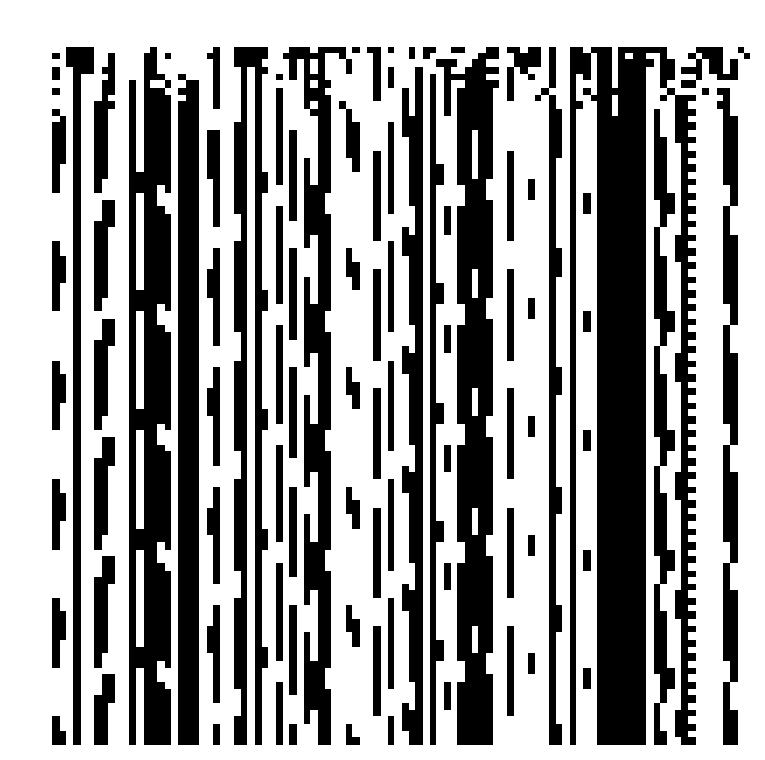
\includegraphics[width=0.5\columnwidth]{method/final-1-noperturb.pdf}
    \label{figure:rbn-noperturb}
  }
  \subfloat[Perturbed]{
    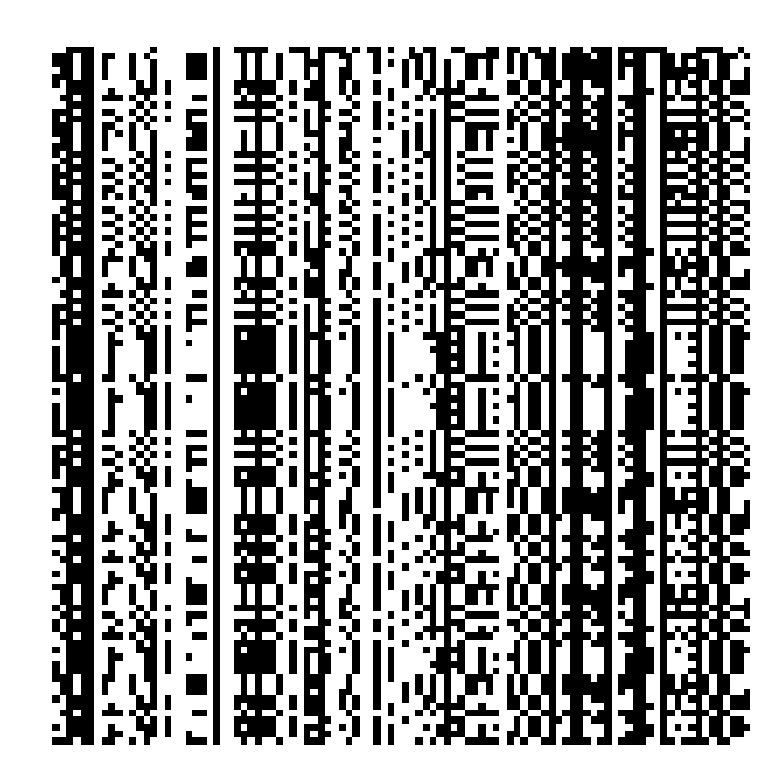
\includegraphics[width=0.5\columnwidth]{method/final-1-perturb.pdf}
    \label{figure:rbn-perturb}
  }
  \caption{The same RBN both perturbed and unperturbed. N=100, K=2, P=0.5, L=50, Initial state=0}
\end{figure}

Should i show the RBN-Reservoir performance in solving time-series tasks here instead of as the first section of results?
